\documentclass[10pt,a4paper]{article}
\usepackage{graphicx}
\usepackage{latexsym}
\usepackage{booktabs}
\usepackage{amsmath}
\usepackage[fleqn]{mathtools}
\usepackage{float}
\usepackage[left=2cm,right=2cm,top=2cm,bottom=2cm]{geometry}

\begin{document}

\begin{titlepage}
	\centering
	{ \huge \scshape National Polytechnic Institute\par}
	{ \Large \scshape  Superior School of Computer Sciences\par }
	\vspace{1cm}
	{\scshape\Large Computer Networks.\par}
	\vspace{1.5cm}
	{\Huge\bfseries Dijkstra's Algorithm.\par}
	\vspace{2cm}
	{\Large\itshape Hernandez Martinez Carlos David.\par}
	{\Large\itshape Grupo: 2cm8. \par}
	\vfill
	{\large \today\par} 
	\vfill
\end{titlepage}


\tableofcontents 
\pagenumbering {arabic}
\pagebreak

\section{Dijkstra's algorithm:}

Using the Dijkstra's algorithm I'll find the Routing table for the Node 1 of the following graph:

\begin{figure}[H]
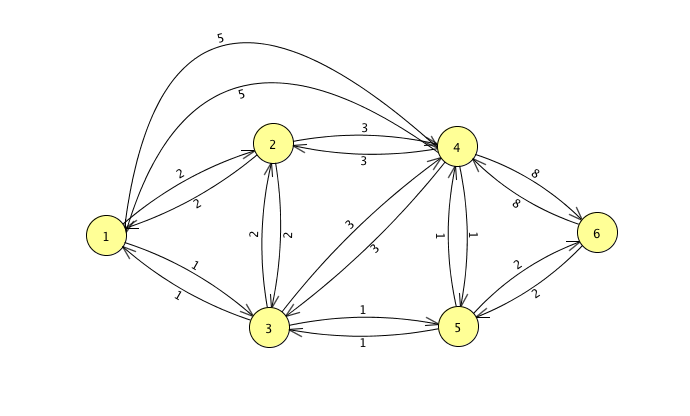
\includegraphics[scale=.6]{Dijkstra.png} 
\centering
\end{figure}

\begin{center}
\begin{tabular}[.5cm]{l c c c c c c c c c c c}
\toprule
M & D2 & PATH & D3 & PATH & D4 & PATH & D5 & PATH & D6 & PATH \\
\midrule
1 & 2 & 1-2 & 1 & 1-3 & 5 & 1-4 & INF & 1-5 & INF & 1-6 \\
\cmidrule{2-11}
1-3 & 2 & 1-2 &  &  & 4 & 1-3-4 & 2 & 1-3-5 & INF & 1-6 \\
\cmidrule{2-11}
1-3-5 & 2 & 1-2 &  &  & 3 & 1-3-5-4 &  &  & 4 & 1-3-5-6 \\
\cmidrule{2-11}
1-3-5-2 &  &  &  &  & 3 & 1-3-5-4 &  &  & 4 & 1-3-5-6 \\
\cmidrule{2-11}
1-3-5-2-4 &  &  &  &  &  &  &  &  & 4 & 1-3-5-6 \\
\cmidrule{2-11}
1-3-5-2-4-6 &  &  &  &  &  &  &  &  &  &  \\
\bottomrule
\linebreak
\end{tabular}
\end{center} 


\subsection{Routing Table:}


\begin{center}
\begin{tabular}[.5cm]{l c c c}
\toprule
Destination & Metric & Next Hop \\
\midrule
1 & 0 & - \\
\cmidrule{1-3}
2 & 2 & 2 \\
\cmidrule{1-3}
3 & 1 & 3 \\
\cmidrule{1-3}
4 & 3 & 3 \\
\cmidrule{1-3}
5 & 2 & 3 \\
\cmidrule{1-3}
6 & 4 & 3 \\
\bottomrule
\linebreak
\end{tabular}
\end{center} 

\pagebreak

\section{Metrics:}

\begin{equation} 
\begin{split}
& For D_{3}\ =\ 1: \\
& D_{2}\ =\ min\ [\ D_{2},\ D_{3}\ +\ d_{2-3}\ ]\ =\ min\ [\ 2,\ 1\ +\ 2\ ]\ =\ 2 \\
& D_{4}\ =\ min\ [\ D_{4},\ D_{3}\ +\ d_{4-3}\ ]\ =\ min\ [\ 5,\ 1\ +\ 3\ ]\ =\ 4 \\
& D_{5}\ =\ min\ [\ D_{5},\ D_{3}\ +\ d_{5-3}\ ]\ =\ min\ [\ INF,\ 1\ +\ 1\ ]\ =\ 2 \\
& D_{6}\ =\ min\ [\ D_{6},\ D_{3}\ +\ d_{6-3}\ ]\ =\ min\ [\ INF,\ 1\ +\ INF\ ]\ =\ INF \\ 
& \\
& For D_{5}\ =\ 2: \\
& D_{2}\ =\ min\ [\ D_{2},\ D_{5}\ +\ d_{2-5}\ ]\ =\ min\ [\ 2,\ 2\ +\ INF\ ]\ =\ 2 \\
& D_{4}\ =\ min\ [\ D_{4},\ D_{5}\ +\ d_{4-5}\ ]\ =\ min\ [\ 4,\ 2\ +\ 1\ ]\ =\ 3 \\
& D_{6}\ =\ min\ [\ D_{6},\ D_{5}\ +\ d_{6-5}\ ]\ =\ min\ [\ INF,\ 2\ +\ 2\ ]\ =\ 4 \\
& \\
& For D_{2}\ =\ 2: \\
& D_{4}\ =\ min\ [\ D_{4},\ D_{2}\ +\ d_{4-2}\ ]\ =\ min\ [\ 3,\ 2\ +\ 3\ ]\ =\ 3 \\
& D_{6}\ =\ min\ [\ D_{6},\ D_{2}\ +\ d_{6-2}\ ]\ =\ min\ [\ 4,\ 2\ +\ INF\ ]\ =\ 4 \\
& \\
& For D_{4}\ =\ 3: \\
& D_{6}\ =\ min\ [\ D_{6},\ D_{4}\ +\ d_{6-2}\ ]\ =\ min\ [\ 4,\ 3\ +\ 8\ ]\ =\ 4 \\
\end{split}
\end{equation}

\end{document}